\onecolumn

\appendix


\section{Meta-prompts} \label{appendix:prompts}



\subsection{Feature Generation Prompt}
In Listing \ref{lst:prompt_generate_features}, we present the feature-generation meta-prompt $Z_{\text{feature}}$, which instructs the LLM to generate a feature set based on the provided feedback.
\label{appendix:feature_generation_prompt}

\begin{listing}[h]
\caption{Prompt for generating node-level features for a GNN binary classifier.}
\label{lst:prompt_generate_features}
\begin{minted}[fontsize=\footnotesize, frame=single, breaklines]{python}
f'''You are an expert in graph neural networks and combinatorial optimization.

Consider the {problem}, defined as ({problem_definition}). 
Propose node-level features for a GNN binary classifier that predicts nodes 
likely to be in the optimal solution.

The heuristic can only select nodes from the reduced candidate set provided 
by the GNN. The goal is to shrink the candidate set while ensuring that the 
heuristic still achieves the same objective value.

Feedback from previous iterations:{explainer_feedback} if {explainer_feedback} else ""
Refinement rules:
1) Keep high-importance features.
2) Avoid proposing features that are too similar to existing or previously failed ones.
3) Replace or remove low-importance features.
4) Add new features inspired by important patterns.
5) Ensure all features are distinct and non-redundant." 


Return the output as a JSON array of objects with keys:
- "feature": feature name in snake_case
- "definition": a one-line definition of how to compute it
- "reason": 1-2 sentences explaining why it is useful

Do not include any text outside the JSON array.
'''
\end{minted}
\end{listing}



\subsection{Summary Generation Prompt}
\label{appendix:summary_generation_prompt}

In Listing \ref{lst:prompt_summarize_feedback}, we present the meta-prompt $Z_{\text{summary}}$, which summarizes the feedback history.

\begin{listing}[h]
\caption{Prompt for summarizing feedback from previous iterations.}
\label{lst:prompt_summarize_feedback}
\begin{minted}[fontsize=\footnotesize, frame=single, breaklines]{python}
f'''You are an expert in graph neural networks and combinatorial optimization.

Summarize the following feedback from previous iterations:
{cumulative_feedback}

Provide a concise summary of the key points and insights.
'''
\end{minted}
\end{listing}


\subsection{Code Generation Prompt}
\label{appendix:code_generation_prompt}

Listing \ref{lst:prompt_extract_feature_single} presents the meta-prompt 
$Z_{code}$, which instructs the LLM to generate efficient feature-extraction code from a given feature definition.



\begin{listing}[!ht]
\caption{Prompt for generating feature-extraction code.}
\label{lst:prompt_extract_feature_single}
\begin{minted}[fontsize=\footnotesize, frame=single, breaklines]{python}




f'''The input is a weighted NetworkX graph G where each node has an attribute weight and an integer variable budget is provided.

Feature name: {feature}
Feature definition: {definition}

"Write Python code for a function extract_feature(G) that computes this feature for ALL nodes in G. The function must return a NumPy array with one value per node, ordered to align with the iteration order of G.nodes()."
"Keep the implementation efficient; avoid expensive computations."
"DO NOT INCLUDE ANY EXPLANATIONS OR COMMENTS."
'''
\end{minted}
\end{listing}



\section{Applications} \label{appendix:applications}

In this section, we formally define the three applications discussed in the paper. A combinatorial optimization problem on a graph can be represented by an undirected graph $G = (V, E)$, where $V$ denotes the set of vertices, $E$ the set of edges, and each node $v \in V$ is associated with a cost $c(v)$.  

\textbf{Maximum Coverage (MaxCov).} Given a budget $k$, the objective is to select a subset of nodes $S \subseteq V$ that maximizes  
\[
f(S) = |\{v \mid v \in S \lor \exists(u, v) \in E, u \in S\}|,
\]
subject to the budget constraint $\sum_{v \in S} c(v) \leq k$.  

Under the size constraint, \llm identifies closed neighborhood size, which includes both the node itself and its immediate neighbors and thus reflects local coverage potential, as the optimal feature. Under the knapsack constraint, the selected features are degree and coverage per cost.

\textbf{Maximum Cut (MaxCut).} Given a budget $k$, the goal is to find a subset of nodes $S \subseteq V$ that maximizes  
\[
f(S) = |\{(u, v) \in E \mid v \in S, u \in V \setminus S\}|,
\]
while satisfying $\sum_{v \in S} c(v) \leq k$.  

Under the size constraint, \llm identifies degree and random cut expectation as the optimal feature set, where random cut expectation measures the expected contribution of a node to the cut value under a randomly generated partition, capturing its average marginal influence. Under the knapsack constraint, the optimal features are degree, weight, degree to weight ratio, normalized degree, neighbor weight sum, and clustering coefficient.

\textbf{Influence Maximization (IM).} Given a budget $k$, edge propagation probabilities $p(u, v)$ for each $(u, v) \in E$, and a cascade model $\mathcal{C}$, the goal is to select a subset $S \subseteq V$ that maximizes the expected influence spread,  
\[
f(S) = \mathbf{E}[\sigma(S)],
\]
where $\sigma(S)$ denotes the number of nodes influenced by $S$, and $\sum_{v \in S} c(v) \leq k$. In our experiments, we adopt the independent cascade model \citep{kempe2003maximizing}, where the edge-level propagation probabilities assigned following the approaches of \citet{ireland2022lense,manchanda2020gcomb}.



Under the size constraint, \llm identifies degree and average incoming activation probability as the optimal features, where average incoming activation probability denotes the mean probability that a node becomes activated by its neighbors, capturing its susceptibility to influence. Under the knapsack constraint, the selected features are degree to weight ratio, outgoing activation probability sum, and in–out degree difference.


% In this section, we formally introduce the three applications mentioned in the paper. A CO problem on graph can be described with an undirected graph $G (V, E)$, where $V$ is the set of vertices, $E$ is the set of edges and each node $v \in V$ is associated with a cost $c(v)$. 

% \textbf{Maximum Cover.} Given a budget $k$ , the goal of this problem is to find a subset of nodes $S \subseteq V$ that maximizes the objective function, $f(S)= |\{v |  v \in S \lor \exists(u,v) \in E , u \in S  \}|$ where $ \sum_{v \in S} c(v) \leq k$.

% \textbf{Maximum Cut (MaxCut).} Given a budget $k$, the goal of this problem is to find a subset of nodes $S \subseteq V$ that maximizes the objective function, $f(S)= |\{ (u,v) \in E: v \in S, u \in V \setminus S \}|$ where $ \sum_{v \in S} c(v) \leq k$.

% \textbf{Influence Maximization (IM).} Given a budget $k$, probabilities $p(u,v)$ on the edges $(u,v)\in E$ and a cascade model $\mathcal{C}$, the goal of this problem is to find a subset of nodes $S \subseteq V$ that maximizes the expected spread, $f(S)= \mathbf{E}[\sigma(S)]$ where $\sigma(S)$ denotes the spread of $S$ and $ \sum_{v \in S} c(v) \leq k$.  For the experiments, we consider the independent cascade model \citep{kempe2003maximizing} and set $p = 0.01$ following \citet{chen2009efficient}. Because relatively large propagation probability $p$ the influence spread is not very sensitive to different algorithms and heuristics, because a giant connected component exists even after removing every edge with probability $1-p$.





\section{Baselines}\label{appendix:baselines}

In this section, we provide detailed descriptions of each algorithm discussed in the paper.




\textbf{GCOMB-P.} For each training graph $G_i = (V, E)$ and a given budget $b$, we begin by ranking all vertices in descending order according to their total outgoing edge weight (or degree, in the case of unweighted graphs). The rank of a vertex $v$, denoted $\text{rank}(v)$, indicates its position in this ordered list, where a lower rank value corresponds to a more influential or connected node.

Next, we employ a stochastic solver $m$ times to generate $m$ different solution sets $\{S^{(1)}, S^{(2)}, \ldots, S^{(m)}\}$ for the same budget $b$. Since the solver introduces randomness, each run may produce a slightly different subset of nodes. Our goal is to identify all nodes that could possibly appear in any of these solutions.

To capture this, we define
\[
r^{G_i}_{b} = \max_{v \in \cup_j S^{(j)}} \text{rank}(v),
\]
which represents the highest-ranked (i.e., least promising) vertex among all nodes selected by the solver across the $m$ runs for graph $G_i$. Intuitively, $r^{G_i}_{b}$ marks the cutoff rank beyond which nodes are unlikely to be part of any optimal or near-optimal solution.

We repeat this computation for every training graph $G_i \in G_{\text{train}}$ and define
\[
r_{b} = \max_{G_i \in G_{\text{train}}} r^{G_i}_{b},
\]
ensuring that $r_b$ generalizes across the entire training distribution for the given budget $b$.

To extend this relationship across different budgets, we compute $r_b$ for a sequence of budgets and record the corresponding pairs $(b, r_b)$. Both the budgets and ranks are then normalized by the total number of nodes in each graph, allowing the learned relationship to generalize across graphs of varying sizes.

During inference, when an unseen budget $b$ is provided, we use linear interpolation over the known $(b, r_b)$ pairs to estimate the corresponding cutoff rank $r_b$. This interpolated value determines the subset of top-ranked nodes to consider as potential solution candidates for the new instance.


% The idea is as follows: For a graph $G_{i} = (V, E)$ from training distribution and a budget of $b$, the vertices are initially sorted into descending order based on the sum of outgoing edge-weight (or degree in an unweighted graph), and $rank(v)$ denotes the position of vertex $v$ in this ordered list. A stochastic solver is used $m$ times to obtain $m$ different solution sets $ \{S^{(1)},S^{(2)},...,S^{(m)}\} $ for budget $b$. The goal here is to predict all nodes that could potentially be part of the solution set.  We define $r^{G_i}_{b}= \max_{v \in \cup_{j} S^{(j)}} rank(v)$ to be the highest rank of all vertices among the vertices in each of the $m$ solution sets. We repeat this process for each graph in the training distribution and define $r_{b} = \max_{G_i \in G_{train}} r^{G_i}_{b}$ for budget $b$. To generalize across budgets, we compute $r_b$ for a series of budgets and obtain $(b,r_b)$ pairs. To generalize across graph sizes, budgets and ranks are normalized with respect to the number of nodes in the graph. During testing, for an unseen budget $b$, linear interpolation is used to predict $r_b$.

% For Max Cover, \citet{manchanda2020gcomb} proposed a novel probabilistic greedy algorithm, and for IM, \citet{manchanda2020gcomb} used IMM \cite{tang2015influence} as the stochastic solvers. 


\textbf{LeNSE.}  \citet{ireland2022lense} proposed a framework for learning to extract a small portion of the original graph that is most likely to contain the optimal solution, enabling efficient downstream optimization using any heuristic. The method first constructs a supervised learning stage followed by a reinforcement learning (RL) stage.

In the first stage, an encoder network is trained to classify subgraphs according to their quality relative to the optimal solution. To build this training data, the optimal solutions are first obtained for all graphs in the training distribution. Then, multiple random subgraphs are generated by sampling different fractions of nodes that overlap with the optimal solution, where each subgraph includes the sampled nodes and their 1-hop neighbors. Each subgraph is assigned to a class based on the ratio between its objective value and that of the original full-graph solution (e.g., high-, medium-, or low-quality). The encoder is trained using these labeled subgraphs so that its embeddings capture structural and functional information correlated with solution quality.

In the second stage, the learned encoder is used to provide the embedding space in which a reinforcement learning agent operates. The RL agent starts from a subgraph induced by a fixed number of randomly selected nodes and their 1-hop neighbors. At each step, the agent updates this subgraph by replacing one vertex with one of its neighbors, thereby navigating the space of subgraphs. The goal of the agent is to discover a subgraph whose embedding is close to those of high-quality (i.e., near-optimal) subgraphs identified during the supervised training phase. In this way, the encoder provides a learned representation of subgraph quality, while the RL agent exploits this representation to efficiently search for promising regions of the graph likely to contain the optimal solution.


% \citet{ireland2022lense} proposed extracting a small portion of the original graph that most likely contains the optimal solution, where the solution can be extracted using any existing heuristics. The idea is as follows: Given a training distribution, extract the optimal solutions for each graph. Next, generate random subgraphs containing different portions of nodes from the optimal solution, where subgraphs are sets of nodes and their 1-hop neighbors. Assign these subgraphs to different classes based on the ratio of the objective function value from the subgraph to that of the original graph. The number of classes depends on the problem and dataset and usually requires domain knowledge.
% In the next step, a reinforcement learning agent is trained to navigate a subgraph induced by a fixed number of random nodes and their 1-hop neighbors, updating the subgraph at each step by replacing a single vertex with its neighbors. By updating the subgraph in this manner, the agent aims to obtain a subgraph close to the optimal subgraph in the embedding space created by the encoder.

\textbf{QuickPrune.} \cite{pmlr-v258-nath25a} proposed a submodularity-based pruning algorithm that filters elements based on their marginal contribution relative to cost, ensuring that uninformative or redundant elements are discarded. To prevent the selected set from growing excessively, the algorithm periodically deletes weaker elements when the accumulated gain exceeds a threshold governed by a deletion parameter. 

\textbf{Submodular Sparsification (SS).}  \citet{zhou2017scaling} introduced a randomized pruning framework for large-scale submodular maximization based on a novel structure called the submodularity graph. The submodularity graph is a weighted directed graph \( G(V, E, w) \) constructed from a normalized submodular function \( f: 2^{V} \rightarrow \mathbb{R}_+ \), where each node in \( V \) represents an element of the ground set, and each directed edge \( (u, v) \in E \) is assigned a weight \( w(u, v) = f(v \mid u) - f(u \mid V \setminus u) \). Since computing all pairwise weights requires quadratic time, the authors proposed a randomized approximation scheme. In each iteration, a random subset of nodes is sampled and temporarily removed from the ground set, while the least influential elements, identified based on their relationships in the sampled subgraph, are discarded. The process continues until the ground set size falls below a predefined threshold, at which point the remaining elements are merged with the pruned subset to form the reduced ground set.
 


% \citet{zhou2017scaling} proposed a randomized pruning method to reduce the submodular maximization problem via a novel concept called the submodularity graph. The submodularity graph is a weighted directed graph \( G(V,E,w) \) defined by a normalized submodular function \( f: 2^{V} \rightarrow \mathcal{R_+} \), where \( V \) is the set of nodes corresponding to the ground set, and each directed edge \( (u,v) \in E \) has weight \( w(u,v) = f(v \mid u) - f(u \mid V \setminus u) \). As computing all edge weights is quadratic in complexity, they proposed a randomized approach. The idea is as follows: Sample a subset of random nodes from the original ground set, remove these random nodes from the ground set at each step, and add them to the pruned ground set. Then, remove a subset of the top elements from the ground set that are deemed unimportant from the sample nodes in that set. After several stages of pruning, when the original ground set size falls below a certain threshold, the remaining elements are merged with the pruned ground set.

\textbf{COMBHelper.}  \citet{tian2024combhelper} proposed a learning-based framework that trains a GNN for vertex classification in combinatorial optimization problems, where the goal is to predict nodes that are likely to be part of the optimal solution. To improve scalability, the authors applied knowledge distillation to transfer knowledge from a larger model to a smaller GNN and incorporated problem-specific weight boosting to further enhance performance.



% \citet{tian2024combhelper} introduced a method to train a GNN for vertex classification in combinatorial problems, predicting nodes likely to be part of the solution. To improve scalability, they applied knowledge distillation to transfer knowledge to a smaller GNN and used problem specific weight boosting to enhance the performance. 




\section{Datasets}\label{appendix:dataset}





Table~\ref{tab:dataset_distribution} summarizes the graph datasets used in our empirical evaluation, including the sizes of their respective training and testing splits for traditional combinatorial optimization problems on graphs. Following \citet{ireland2022lense}, we determine the proportion of edges from each original graph allocated to the training and testing sets.



% In Table \ref{tab:dataset_distribution}, we list the graphs used in our empirical evaluations along with the sizes of the respective training and testing splits for the traditional CO problems on graphs. We follow \citet{ireland2022lense} to determine what percentage of the original graph edges was used for training and testing.

\begin{table}[h]
\centering
\caption{The real-world graphs used to perform our experiments. 
% For each graph, we provide the corresponding size of the training and
% testing sets; in brackets we indicate the percentage of edges taken from the original graph for training purposes with the remaining edges
% being used to form the test graph.
}

\vspace{1em}
\begin{tabular}{|c|c|c|c|c|}
\hline
         & \multicolumn{2}{c|}{Train Size}        & \multicolumn{2}{c|}{Test Size}           \\ \cline{2-5} 
Graph    & \multicolumn{1}{c|}{Vertices} & Edges  & \multicolumn{1}{c|}{Vertices} & Edges    \\ \hline
Facebook & 3847                          & $26470 (30\%)$  & 4002                          & 61764    \\
Wiki     & 4891                          & $30228 (30\%)$  & 6358                          & 70534    \\
Deezer   & 48870                         & $149460 (30\%)$& 53511                         & 348742   \\
SlashDot & 47546                         & $140566 (30\%)$& 67640                         & 327988   \\
Twitter  & 55827                         & $134229 (10\%)$& 80712                         & 1208067  \\
DBLP     & 63004                         & $41994 (10\%)$ & 315305                        & 1007872  \\
YouTube  & 185193                        & $179257 (06\%)$ & 1098104                       & 2808367  \\
Skitter  & 147604                        & $110952 (01\%)$ & 1694318                       & 10984346 \\ \hline
\end{tabular}

\label{tab:dataset_distribution}
\end{table}



\section{Network Architectures And Hyper-parameters} \label{appendix:network}

\textbf{Beam Search.} Beam search hyperparameters are determined using a grid search over $\beta$, $\gamma$, and $D$  for Maximum Coverage problem. We select $\beta = 3$, $\gamma = 2$, and $D = 5$ based on their stable performance across datasets and constraints, avoiding over-specialization to any single problem. This configuration is then fixed across all reported experiments.

\textbf{Training Data Generation.} For feature space search, we use the Holme-Kim random graph model with $n = 10{,}000$ nodes and hyperparameters $m = 4$ and $p = 0.01$ for training and validation.

\textbf{LLM Settings.} We run with GPT-5-nano and LLaMA-3.3-70B-Instruct with default parameters provided in the documentation.

\textbf{GNN.} The architecture consists of two layers, each containing a graph convolutional layer with ReLU
activation and $16$ hidden channels.

\textbf{Timeout Mechanism.} We set the cutoff time as 5 seconds to bound feature-space exploration and ensure practical runtime.

\textbf{Semi-supervised Learning.} During training, we employ pseudo-labeling with a confidence threshold of $\delta=0.90$ and select the top $k=100$ most confident predictions at each iteration after a warm-up period of 500 epochs.
.

\textbf{Testing Settings.} We adopt a progressive expansion strategy to determine an effective candidate ground set for heuristic evaluation. Starting with the top $500$ nodes ranked by their predicted probabilities, the heuristic is first applied to obtain an initial objective value. The candidate set is then progressively expanded to include the top $1,000$, $2,000$, and $5,000$ nodes, respectively. After each expansion, the heuristic is re-evaluated, and the relative improvement in the objective value is measured. The process continues until the improvement falls below $1\%$, at which point the current subset is selected as the final ground set. This procedure ensures a balance between computational efficiency and solution quality.



\section{Ablation Study} \label{appendix:ablation}

We conduct an ablation study to analyze the contribution of the major components of \llm. Specifically, we evaluate the following variants of our framework using GPT-5-nano.

\begin{itemize}
    \item \textbf{Single-shot prompt:} A single LLM query is used to generate features without any iterative refinement or feedback.

    \item \textbf{Simple feedback loop with performance feedback:} The LLM iteratively refines features based solely on downstream performance metrics from the learned pruning model.

    \item \textbf{Simple feedback loop with performance feedback and feature importance:} In addition to performance metrics, feature-importance scores from the classifier are provided to guide feature refinement.

    \item \textbf{Beam search:} Multiple candidate feature sets are maintained at each iteration, with beam expansion guided by performance and feature-importance feedback.
\end{itemize}

To ensure a fair comparison, all variants use the same number of API calls. In Figure~\ref{fig:abalation}, we report the combined metric across three CO problems under knapsack constraints. The results show that beam search consistently achieves higher and more stable performance, with median values close to $1.0$ and minimal variance across runs.


% An ablation study is carried out to provide a better understanding of the contribution of major components in EoH. We consider the following varients.

% \begin{itemize}
%     \item Single Shot Prompt:

%     \item Simple Feed Back Loop with performance feedback:

%     \item Simple Feedback loop with performance feedback and feature importance:

%     \item Beam Search:
% \end{itemize}

% To have a fair comparison, all the variants use the same number of API calls. In Figure ~\ref{fig:abalation}, we present the combined metric for the three CO problems under knapsack constraints . The results clearly indicate that Beam Search consistently achieves higher and more stable performance, with median values close to $1.0$ and minimal variance across runs.


% In Figure ~\ref{fig:abalation}, we present the combined metric for the three CO problems over five runs of beam search using the aforementioned parameters and simple feedback with $10$ iterations. The results clearly indicate that Beam Search consistently achieves higher and more stable performance, with median values close to $1.0$ and minimal variance across runs. In contrast, simple feedback exhibits much larger variability, particularly for Maximum Coverage, where performance drops sharply in several runs. This suggests that the beam-based exploration strategy enables a more reliable feature set and avoids the instability observed in the simpler feedback mechanism.



\begin{figure}[h]
    \centering
    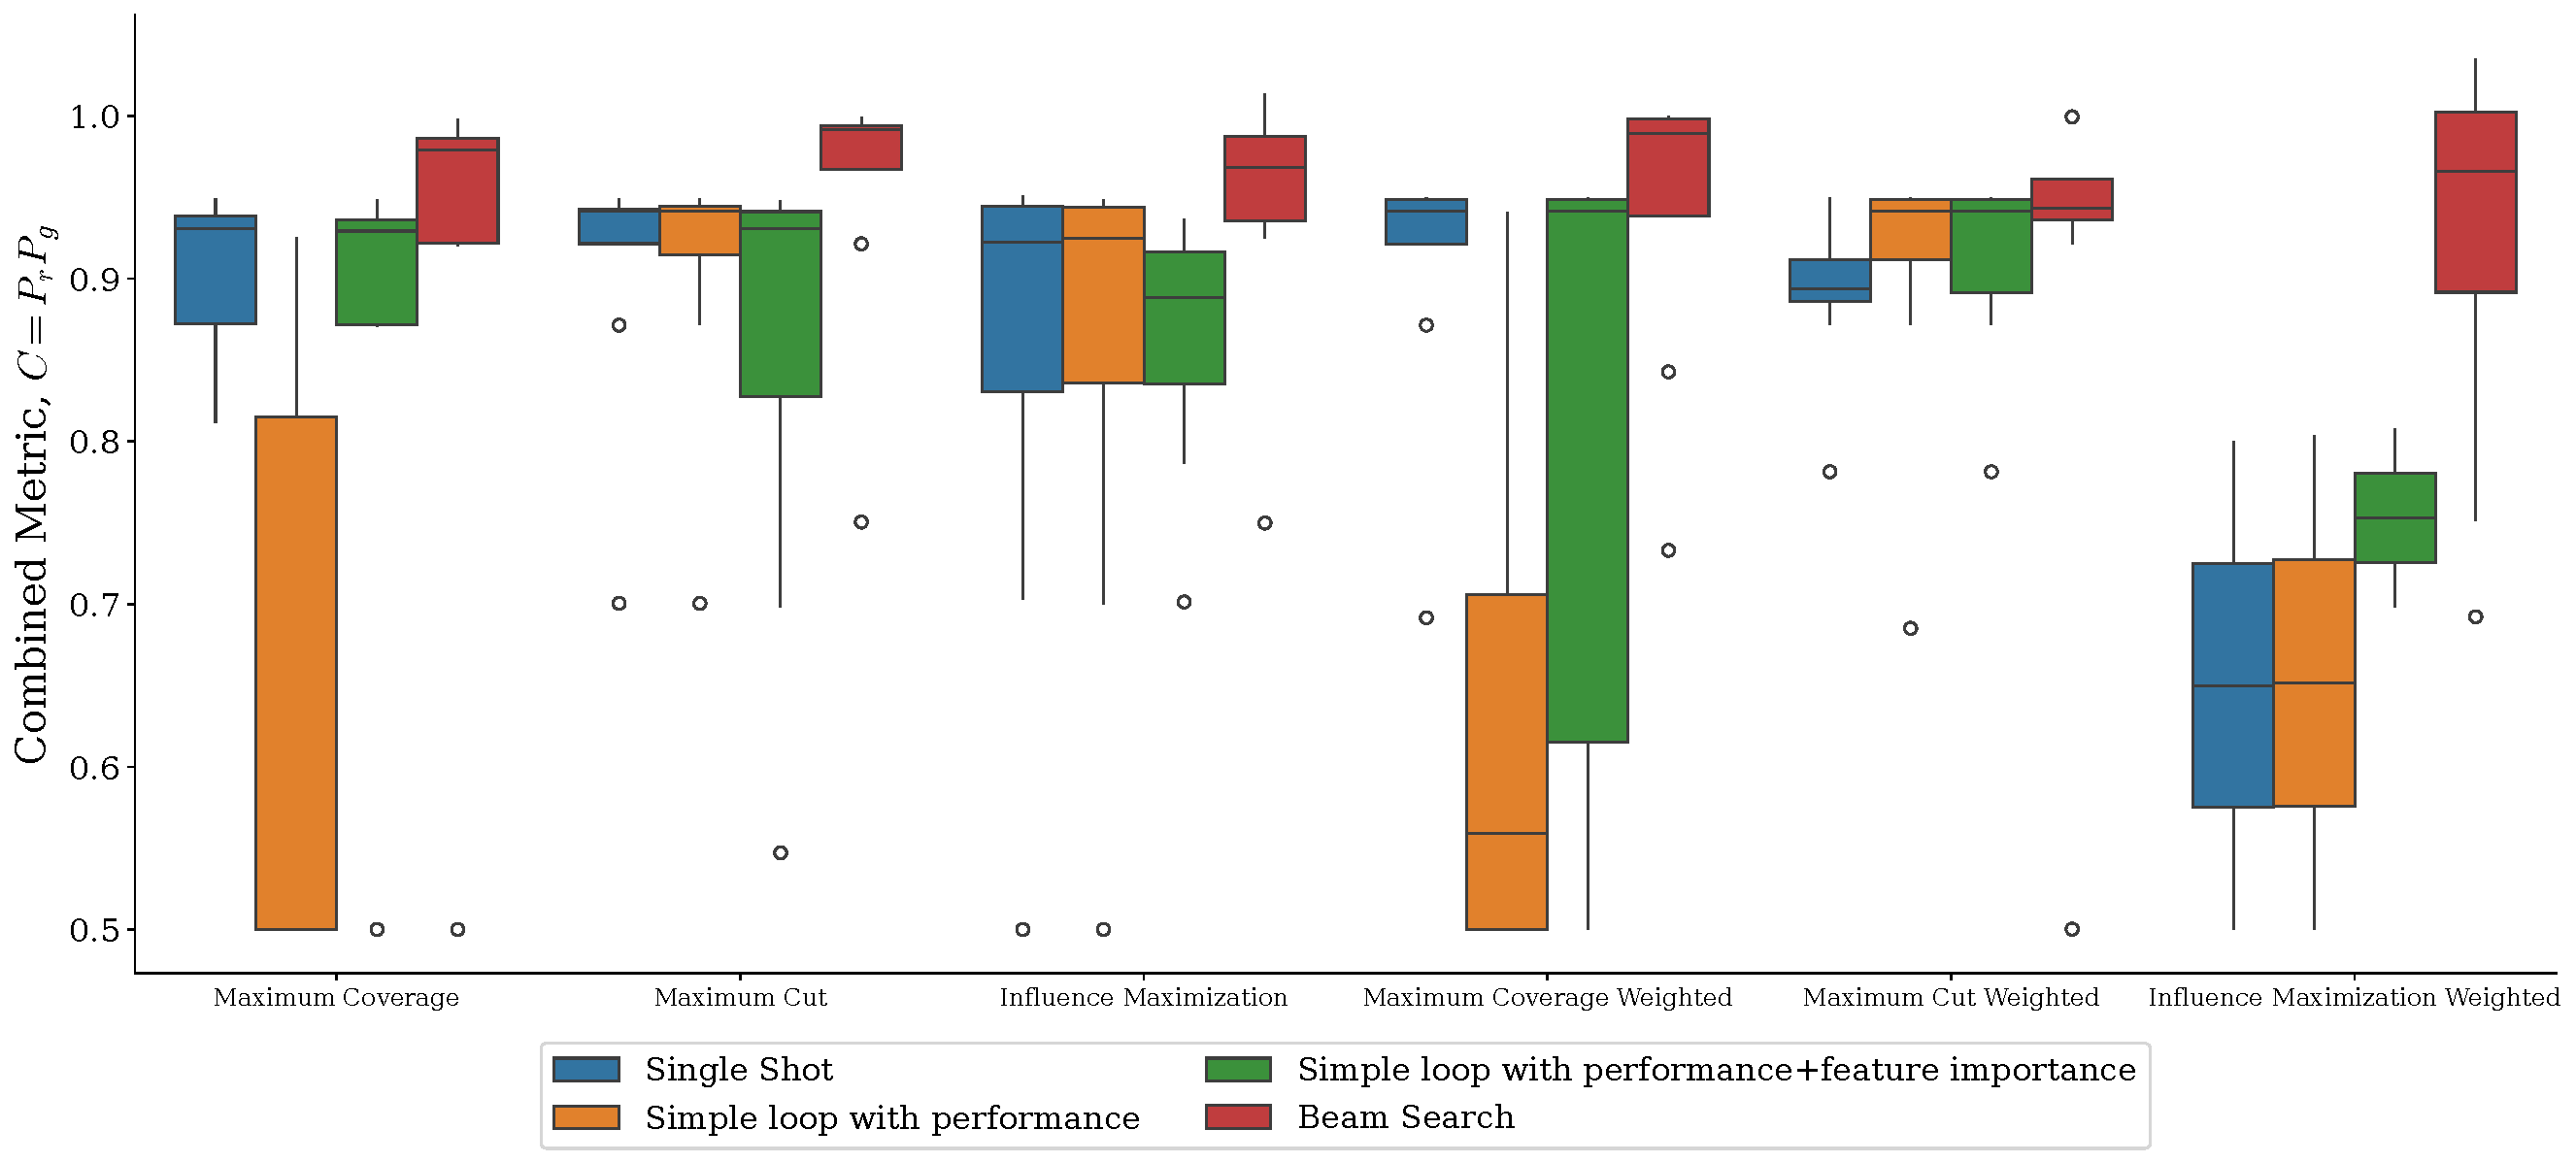
\includegraphics[width=\linewidth]{figures/ablation.pdf}
    \caption{Performance comparison of different variants of \llm.}
    \label{fig:abalation}
\end{figure}

\section{Additional Tables and Plots} \label{appendix:additional}




\subsection{Evaluation on Size Constraint}

In Table \ref{tab:multi_problem_algos_remain}, we represent the performance of the pruning algorithms on Maximum Coverage under size constraint. 

\begin{table*}[h]
\centering
\caption{Comparison of pruning algorithms for size-constraint experiments. Highlighted are the results ranked \textbf{\textcolor{lightred}{first}}, \textbf{\textcolor{lightblue}{second}} , and \textbf{\textcolor{lightgreen}{third}}. *Values are reported from \cite{ireland2022lense,pmlr-v258-nath25a}. “--” indicates that the corresponding algorithm obtained no reasonable result.}
\vspace{1em}
\label{tab:multi_problem_algos_remain}
\resizebox{\textwidth}{!}{%
\begin{tabular}{lccc|ccc|ccc|ccc|ccc|ccc}
\toprule
 & \multicolumn{6}{c}{\textbf{Classical Approach}} & \multicolumn{12}{c}{\textbf{Learning-Based Approach}} \\
\cmidrule(lr){2-7} \cmidrule(lr){8-19}
 \textbf{Dataset} & \multicolumn{3}{c}{\text{\textsc{QuickPrune}}} & \multicolumn{3}{c}{\text{SS}} & \multicolumn{3}{c}{\textbf{LLM2Prune}} & \multicolumn{3}{c}{\text{GCOMB-P*}} & \multicolumn{3}{c}{\textsc{LeNSE*}} & \multicolumn{3}{c}{\textsc{COMBHelper*}} \\
& \textbf{$P_r$} & \textbf{$P_g$} & \textbf{$C$} & \textbf{$P_r$} & \textbf{$P_g$} & \textbf{$C$} & \textbf{$P_r$} & \textbf{$P_g$} & \textbf{$C$} & \textbf{$P_r$} & \textbf{$P_g$} & \textbf{$C$} & \textbf{$P_r$} & \textbf{$P_g$} & \textbf{$C$} & \textbf{$P_r$} & \textbf{$P_g$} & \textbf{$C$} \\
\midrule
\multicolumn{19}{c}{\textbf{Maximum Coverage}} \\
 \midrule
Facebook & 1.0000 & 0.9953 & \textbf{\textcolor{lightred}{0.9953}} & 0.9884 & 0.9027 & \textbf{\textcolor{lightblue}{0.8922}} & 0.9966 & 0.5002 & \textbf{\textcolor{lightgreen}{0.4985}} & 0.9270 & 0.0700 & 0.0649 & 0.9660 & 0.0700 & 0.0676 & 1.0000 & 0.3840 & 0.3840 \\
DBLP & 0.9951 & 0.9957 & \textbf{\textcolor{lightred}{0.9908}} & 0.9945 & 0.9963 & \textbf{\textcolor{lightblue}{0.9908}} & 1.0000 & 0.9841 & \textbf{\textcolor{lightgreen}{0.9841}} & 0.9990 & 0.0300 & 0.0300 & 0.9900 & 0.9000 & 0.8910 & 1.0000 & 0.1818 & 0.1818 \\
Deezer & 0.9606 & 0.9797 & \textbf{\textcolor{lightgreen}{0.9411}} & 0.9870 & 0.9855 & \textbf{\textcolor{lightblue}{0.9727}} & 0.9930 & 0.9813 & \textbf{\textcolor{lightred}{0.9745}} & 0.9940 & 0.1300 & 0.1292 & 0.9790 & 0.7500 & 0.7343 & 1.0000 & 0.7278 & 0.7278 \\
Slashdot & 1.0000 & 0.9925 & \textbf{\textcolor{lightred}{0.9925}} & 0.9824 & 0.9889 & 0.9715 & 0.9914 & 0.9926 & \textbf{\textcolor{lightgreen}{0.9840}} & 1.0000 & 0.0200 & 0.0200 & 0.9790 & 0.6900 & 0.6755 & 1.0000 & 0.9844 & \textbf{\textcolor{lightblue}{0.9844}} \\
Wiki & 0.9998 & 0.9422 & \textbf{\textcolor{lightred}{0.9420}} & 0.9559 & 0.9346 & \textbf{\textcolor{lightgreen}{0.8934}} & 0.9988 & 0.9214 & \textbf{\textcolor{lightblue}{0.9202}} & 0.9900 & 0.0300 & 0.0297 & 1.0940 & 0.3400 & 0.3720 & 1.0000 & 0.4528 & 0.4528 \\
Twitter & 0.9929 & 0.9911 & \textbf{\textcolor{lightred}{0.9841}} & 0.9306 & 0.9893 & \textbf{\textcolor{lightgreen}{0.9206}} & 0.9834 & 0.9381 & \textbf{\textcolor{lightblue}{0.9225}} & 0.9970 & 0.1700 & 0.1695 & 0.9890 & 0.3300 & 0.3264 & 1.0000 & 0.5654 & 0.5654 \\
YouTube & 1.0000 & 0.9995 & \textbf{\textcolor{lightred}{0.9995}} & 0.9999 & 0.9987 & \textbf{\textcolor{lightblue}{0.9986}} & 0.9993 & 0.9991 & \textbf{\textcolor{lightgreen}{0.9984}} & 0.9980 & 0.0700 & 0.0699 & 0.9820 & 0.7900 & 0.7758 & 1.0000 & 0.9572 & 0.9572 \\
Skitter & 0.9985 & 0.9997 & \textbf{\textcolor{lightred}{0.9982}} & 0.9857 & 0.9991 & \textbf{\textcolor{lightgreen}{0.9848}} & 0.9958 & 0.9970 & \textbf{\textcolor{lightblue}{0.9928}} & 0.9990 & 0.1000 & 0.0999 & 0.9760 & 0.7000 & 0.6832 & -- & -- & -- \\
\midrule

\bottomrule
\end{tabular}
}
\end{table*}


\subsection{Evaluation on Knapsack Constraint}
In Table \ref{tab:multi_problem_knapsack}, we represent the performance of the pruning algorithms on Maximum Coverage under size constraint.
\begin{table*}[h]
\centering
\caption{Comparison of pruning algorithms for size-constraint experiments. Highlighted are the results ranked \textbf{\textcolor{lightred}{first}}, \textbf{\textcolor{lightblue}{second}} , and \textbf{\textcolor{lightgreen}{third}}. *Values are reported from \cite{pmlr-v258-nath25a}.}
\vspace{1em}
\label{tab:multi_problem_knapsack}

\begin{tabular}{l|ccc|ccc|ccc}
\toprule
\textbf{Dataset} & \multicolumn{3}{c|}{\textsc{QuickPrune}} & \multicolumn{3}{c|}{\textsc{TOP-k}} & \multicolumn{3}{c}{\textsc{LLM2Prune}} \\
 & \textbf{$P_r$} & \textbf{$P_g$} & \textbf{$C$} & \textbf{$P_r$} & \textbf{$P_g$} & \textbf{$C$} & \textbf{$P_r$} & \textbf{$P_g$} & \textbf{$C$} \\
\midrule
\multicolumn{10}{c}{\textbf{Maximum Coverage Weighted}} \\
 \midrule
Facebook & 0.9725 & 0.9871 & \textbf{\textcolor{lightred}{0.9600}} & 0.5505 & 0.9871 & \textbf{\textcolor{lightgreen}{0.5434}} & 0.9771 & 0.7501 & \textbf{\textcolor{lightblue}{0.7330}} \\
DBLP & 0.8450 & 0.9997 & \textbf{\textcolor{lightblue}{0.8447}} & 0.7150 & 0.9997 & \textbf{\textcolor{lightgreen}{0.7148}} & 1.0000 & 0.9984 & \textbf{\textcolor{lightred}{0.9984}} \\
Deezer & 0.8750 & 0.9983 & \textbf{\textcolor{lightgreen}{0.8735}} & 0.9150 & 0.9983 & \textbf{\textcolor{lightblue}{0.9134}} & 1.0000 & 0.9907 & \textbf{\textcolor{lightred}{0.9907}} \\
Slashdot & 0.8950 & 0.9988 & \textbf{\textcolor{lightblue}{0.8939}} & 0.5700 & 0.9988 & \textbf{\textcolor{lightgreen}{0.5693}} & 1.0000 & 0.9704 & \textbf{\textcolor{lightred}{0.9704}} \\
Wiki & 0.9400 & 0.9851 & \textbf{\textcolor{lightred}{0.9260}} & 0.7550 & 0.9851 & \textbf{\textcolor{lightgreen}{0.7438}} & 1.0000 & 0.8427 & \textbf{\textcolor{lightblue}{0.8427}} \\
Twitter & 0.8700 & 0.9987 & \textbf{\textcolor{lightblue}{0.8689}} & 0.5950 & 0.9987 & \textbf{\textcolor{lightgreen}{0.5942}} & 1.0000 & 0.9876 & \textbf{\textcolor{lightred}{0.9876}} \\
YouTube & 0.9150 & 0.9999 & \textbf{\textcolor{lightblue}{0.9149}} & 0.5200 & 0.9999 & \textbf{\textcolor{lightgreen}{0.5199}} & 1.0000 & 0.9982 & \textbf{\textcolor{lightred}{0.9982}} \\
Skitter & 0.9050 & 0.9999 & \textbf{\textcolor{lightblue}{0.9049}} & 0.8150 & 0.9999 & \textbf{\textcolor{lightgreen}{0.8149}} & 1.0000 & 0.9997 & \textbf{\textcolor{lightred}{0.9997}} \\
\midrule
\multicolumn{10}{c}{\textbf{Maximum Cut Weighted}} \\
 \midrule
Facebook & 0.9899 & 0.9666 & \textbf{\textcolor{lightblue}{0.9568}} & 1.0000 & 0.9666 & \textbf{\textcolor{lightred}{0.9666}} & 1.0000 & 0.5002 & \textbf{\textcolor{lightgreen}{0.5002}} \\
DBLP & 0.9500 & 0.9999 & \textbf{\textcolor{lightred}{0.9499}} & 0.4300 & 0.9999 & \textbf{\textcolor{lightgreen}{0.4300}} & 0.9500 & 0.9984 & \textbf{\textcolor{lightblue}{0.9485}} \\
Deezer & 0.9600 & 0.9985 & \textbf{\textcolor{lightred}{0.9586}} & 0.8000 & 0.9985 & \textbf{\textcolor{lightgreen}{0.7988}} & 0.9500 & 0.9907 & \textbf{\textcolor{lightblue}{0.9411}} \\
Slashdot & 0.9700 & 0.9991 & \textbf{\textcolor{lightred}{0.9691}} & 0.6700 & 0.9991 & \textbf{\textcolor{lightgreen}{0.6694}} & 0.9500 & 0.9926 & \textbf{\textcolor{lightblue}{0.9430}} \\
Wiki & 0.9600 & 0.9928 & \textbf{\textcolor{lightred}{0.9531}} & 0.5100 & 0.9928 & \textbf{\textcolor{lightgreen}{0.5063}} & 1.0000 & 0.9214 & \textbf{\textcolor{lightblue}{0.9214}} \\
Twitter & 0.9500 & 0.9996 & \textbf{\textcolor{lightred}{0.9496}} & 0.2900 & 0.9996 & \textbf{\textcolor{lightgreen}{0.2899}} & 0.9500 & 0.9938 & \textbf{\textcolor{lightblue}{0.9441}} \\
YouTube & 0.9700 & 0.9999 & \textbf{\textcolor{lightblue}{0.9699}} & 0.7300 & 0.9999 & \textbf{\textcolor{lightgreen}{0.7299}} & 1.0000 & 0.9995 & \textbf{\textcolor{lightred}{0.9995}} \\
Skitter & 0.9700 & 0.9999 & \textbf{\textcolor{lightgreen}{0.9699}} & 1.0000 & 0.9999 & \textbf{\textcolor{lightred}{0.9999}} & 1.0000 & 0.9994 & \textbf{\textcolor{lightblue}{0.9994}} \\
\midrule
\multicolumn{10}{c}{\textbf{Influence Maximization Weighted}} \\
 \midrule
Facebook & 0.9934 & 0.9148 & \textbf{\textcolor{lightred}{0.9088}} & 0.9934 & 0.9148 & \textbf{\textcolor{lightblue}{0.9088}} & 1.0014 & 0.7501 & \textbf{\textcolor{lightgreen}{0.7512}} \\
DBLP & 1.0000 & 0.9958 & \textbf{\textcolor{lightred}{0.9958}} & 1.0000 & 0.9958 & \textbf{\textcolor{lightblue}{0.9958}} & 0.9646 & 0.9937 & \textbf{\textcolor{lightgreen}{0.9585}} \\
Deezer & 1.0000 & 0.9820 & \textbf{\textcolor{lightred}{0.9820}} & 1.0000 & 0.9820 & \textbf{\textcolor{lightblue}{0.9820}} & 0.9923 & 0.9813 & \textbf{\textcolor{lightgreen}{0.9738}} \\
Slashdot & 0.9132 & 0.9868 & \textbf{\textcolor{lightgreen}{0.9011}} & 1.0120 & 0.9868 & \textbf{\textcolor{lightred}{0.9986}} & 1.0067 & 0.9852 & \textbf{\textcolor{lightblue}{0.9918}} \\
Wiki & 0.9660 & 0.8774 & \textbf{\textcolor{lightblue}{0.8476}} & 1.0000 & 0.8774 & \textbf{\textcolor{lightred}{0.8774}} & 1.0098 & 0.6854 & \textbf{\textcolor{lightgreen}{0.6922}} \\
Twitter & 0.9121 & 0.9986 & \textbf{\textcolor{lightgreen}{0.9108}} & 0.9689 & 0.9986 & \textbf{\textcolor{lightred}{0.9675}} & 1.0005 & 0.9381 & \textbf{\textcolor{lightblue}{0.9385}} \\
YouTube & 0.9171 & 0.9994 & \textbf{\textcolor{lightgreen}{0.9165}} & 0.9502 & 0.9994 & \textbf{\textcolor{lightblue}{0.9496}} & 1.0400 & 0.9954 & \textbf{\textcolor{lightred}{1.0353}} \\
Skitter & 0.8291 & 0.9999 & \textbf{\textcolor{lightgreen}{0.8290}} & 0.9391 & 0.9999 & \textbf{\textcolor{lightblue}{0.9390}} & 1.0345 & 0.9997 & \textbf{\textcolor{lightred}{1.0342}} \\
\midrule
\bottomrule
\end{tabular}

\end{table*}

\subsection{Runtime}\label{appendix:runtime}

\textcolor{blue}{Table~\ref{tab:runtime_absolute} reports the absolute inference runtimes for all evaluated algorithms on the Influence Maximization problem under the size constraint. All algorithms are evaluated using the same computational resources (identical numbers of threads and GPUs) to ensure a fair comparison. The only exception is SS, which requires additional threads on large graphs.}

\llm{} \textcolor{blue}{is 1-4 orders of magnitude faster than classical methods on larger graphs, completing inference in under 3 seconds even on Skitter.}

\begin{table}[h]
\centering
\caption{Absolute inference runtime (seconds) for Influence Maximization under size constraint. *SS uses additional threads on large graphs to speed up pruning; all other algorithms use the same number of threads and GPUs.}
\label{tab:runtime_absolute}
\resizebox{\textwidth}{!}{%
\begin{tabular}{lcccccccc}
\toprule
\textbf{Algorithm} & \textbf{Facebook} & \textbf{Wiki} & \textbf{Deezer} & \textbf{Slashdot} & \textbf{Twitter} & \textbf{DBLP} & \textbf{YouTube} & \textbf{Skitter} \\
\midrule
\llm      & 0.194  & 0.203  & 0.235  & 0.257   & 0.314    & 0.458   & 1.118    & 2.420     \\
\qp       & 1.860  & 41.960 & 1.100  & 226.000 & 3219.040 & 222.760 & 658.320  & 5109.000  \\
SS*       & 24.960 & 86.424 & 11.371 & 102.259 & 1242.836 & 118.537 & 3652.793 & 10433.744 \\
GCOMB-P   & 0.002  & 0.004  & 0.023  & 0.035   & 0.051    & 0.205   & 0.515    & 0.980     \\
\lense    & 31.453 & 36.476 & 42.164 & 44.193  & 81.610   & 49.286  & 238.906  & 1607.605  \\
\bottomrule
\end{tabular}%
}
\end{table}

\textcolor{blue}{Table~\ref{tab:runtime_breakdown} breaks down the total inference time of \llm into feature extraction and GNN inference components.}

\begin{table}[h!]
\centering
\caption{Runtime breakdown of \llm for Influence Maximization under size constraint.}
\label{tab:runtime_breakdown}
\begin{tabular}{lcccc}
\toprule
\textbf{Dataset} & \textbf{Feature Extraction (s)} & \textbf{GNN Inference (s)} & \textbf{Total (s)} \\
\midrule
Facebook & 0.006 & 0.188 & 0.194 \\
Wiki     & 0.008 & 0.195 & 0.203 \\
Deezer   & 0.058 & 0.177 & 0.235 \\
Slashdot & 0.063 & 0.193 & 0.257 \\
Twitter  & 0.138 & 0.176 & 0.314 \\
DBLP     & 0.284 & 0.175 & 0.458 \\
YouTube  & 0.942 & 0.176 & 1.118 \\
Skitter  & 2.195 & 0.225 & 2.420 \\
\bottomrule
\end{tabular}
\end{table}


% In Figure \ref{fig:run_time_breakdown}, we separate the total pruning time into feature extraction and GNN inference components. As the dataset size increases, both components grow approximately linearly, with GNN inference contributing slightly more to the total runtime on larger graphs such as YouTube and Skitter. Overall, the pruning stage remains efficient, completing within about $10$ seconds even for the largest datasets.

% \begin{figure}[h!]
%     \centering
%     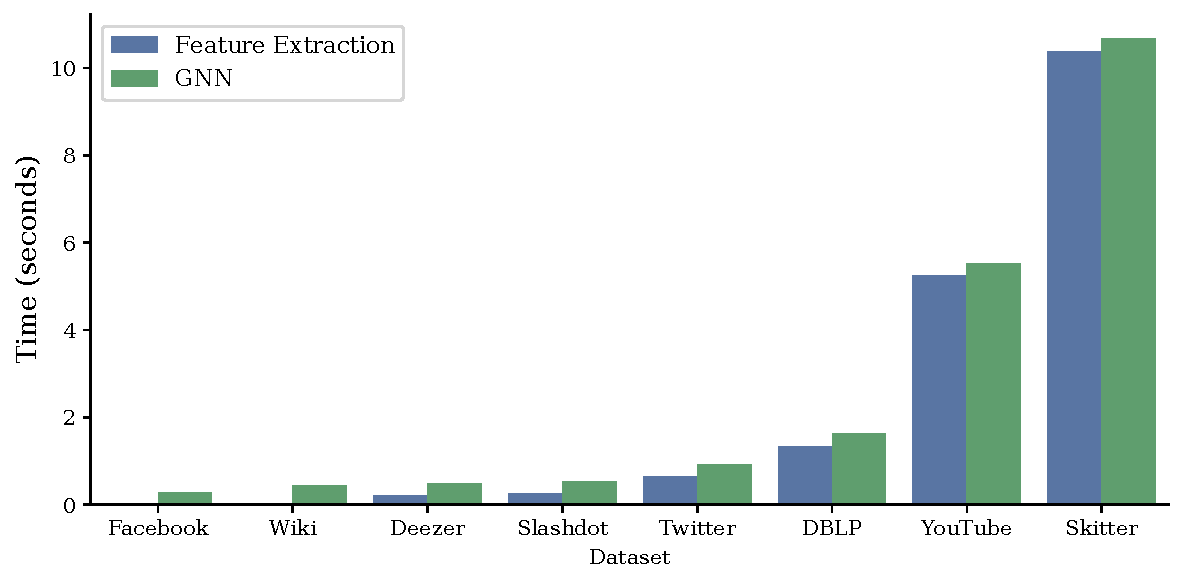
\includegraphics[width=0.8\linewidth]{figures/Maximum Coverage Weighted_runtime_barplot.pdf}
%     \caption{Runtime breakdown for the Maximum Coverage Problem under size constraint.}
%     \label{fig:run_time_breakdown}
% \end{figure}

\subsection{Multi-budget Analysis.} \label{appendix:multibudget}

In Table \ref{tab:multibudget_size}, we present the pruning approximation ratio ($P_r$) across a range of budgets under the size constraint following \cite{ireland2022lense}. The results exhibit similar trends for the knapsack constraint.

\begin{table}[h!]
\centering
\caption{Performance of \llm across a range of budgets across three CO problems under size constraint.}
\label{tab:multibudget_size}
\begin{tabular}{lcccccc}
\toprule
\multicolumn{7}{c}{\textbf{Maximum Coverage}} \\
\midrule
\textbf{Dataset} & 1 & 10 & 25 & 50 & 75 & 100 \\
\midrule
Facebook & 1.0000 & 1.0000 & 0.9982 & 0.9974 & 0.9959 & 0.9966 \\
Wiki & 1.0000 & 1.0000 & 1.0000 & 1.0000 & 0.9997 & 0.9988 \\
Deezer & 1.0000 & 1.0000 & 1.0000 & 0.9972 & 0.9962 & 0.9930 \\
Slashdot & 1.0000 & 1.0000 & 1.0000 & 0.9992 & 0.9963 & 0.9914 \\
Twitter & 1.0000 & 1.0000 & 1.0000 & 0.9993 & 0.9961 & 0.9834 \\
DBLP & 1.0000 & 1.0000 & 1.0000 & 1.0000 & 1.0000 & 1.0000 \\
YouTube & 1.0000 & 1.0000 & 1.0000 & 1.0000 & 1.0000 & 0.9993 \\
Skitter & 1.0000 & 1.0000 & 1.0000 & 1.0000 & 0.9974 & 0.9958 \\
\midrule
\multicolumn{7}{c}{\textbf{Maximum Cut}} \\
\midrule
\textbf{Dataset} & 1 & 10 & 25 & 50 & 75 & 100 \\
\midrule
Facebook & 1.0000 & 1.0000 & 1.0000 & 1.0000 & 1.0004 & 1.0004 \\
Wiki & 1.0000 & 1.0000 & 1.0000 & 1.0000 & 1.0000 & 1.0000 \\
Deezer & 1.0000 & 1.0000 & 1.0000 & 1.0000 & 1.0000 & 0.9999 \\
Slashdot & 1.0000 & 1.0000 & 1.0000 & 1.0000 & 1.0000 & 1.0000 \\
Twitter & 1.0000 & 1.0000 & 1.0000 & 1.0000 & 1.0000 & 1.0000 \\
DBLP & 1.0000 & 1.0000 & 1.0000 & 0.9984 & 0.9979 & 0.9981 \\
YouTube & 1.0000 & 1.0000 & 1.0000 & 1.0000 & 1.0000 & 1.0000 \\
Skitter & 1.0000 & 1.0000 & 1.0000 & 1.0000 & 0.9994 & 0.9966 \\
\midrule
\multicolumn{7}{c}{\textbf{Influence Maximization}} \\
\midrule
\textbf{Dataset} & 1 & 10 & 25 & 50 & 75 & 100 \\
\midrule
Facebook & 0.9802 & 0.9911 & 0.9905 & 0.9933 & 1.0035 & 1.0047 \\
Wiki & 0.9904 & 1.0181 & 1.0010 & 1.0057 & 1.0000 & 1.0014 \\
Deezer & 1.0015 & 1.0088 & 0.9738 & 0.9870 & 0.9784 & 0.9871 \\
Slashdot & 1.0225 & 1.0076 & 0.9967 & 1.0068 & 1.0079 & 1.0104 \\
Twitter & 0.9997 & 0.9937 & 0.9869 & 0.9819 & 0.9790 & 0.9695 \\
DBLP & 0.9490 & 0.9552 & 0.9653 & 0.9847 & 0.9903 & 0.9941 \\
YouTube & 0.9999 & 1.0036 & 0.9976 & 1.0082 & 1.0014 & 0.9995 \\
Skitter & 0.9998 & 0.9995 & 0.9992 & 0.9989 & 0.9991 & 1.0006 \\
\midrule
\bottomrule
\end{tabular}
\end{table}



\subsection{Comparison of \llm with different LLMs}

We evaluate the robustness of \llm with respect to the choice of the underlying LLM by comparing two representative LLMs: GPT-5-nano and LLaMA-3.3-70B-Instruct. Both models are used identically within the framework to propose features, generate executable code, and summarize feedback, while all downstream components, hyperparameters, and evaluation protocols are kept fixed.

Figure~\ref{fig:models} reports the combined performance metric across all graph optimization tasks under size constraints. The results show that \llm achieves comparable performance with both LLMs, indicating that the framework is not sensitive to a specific model choice. 


\begin{figure}
    \centering
    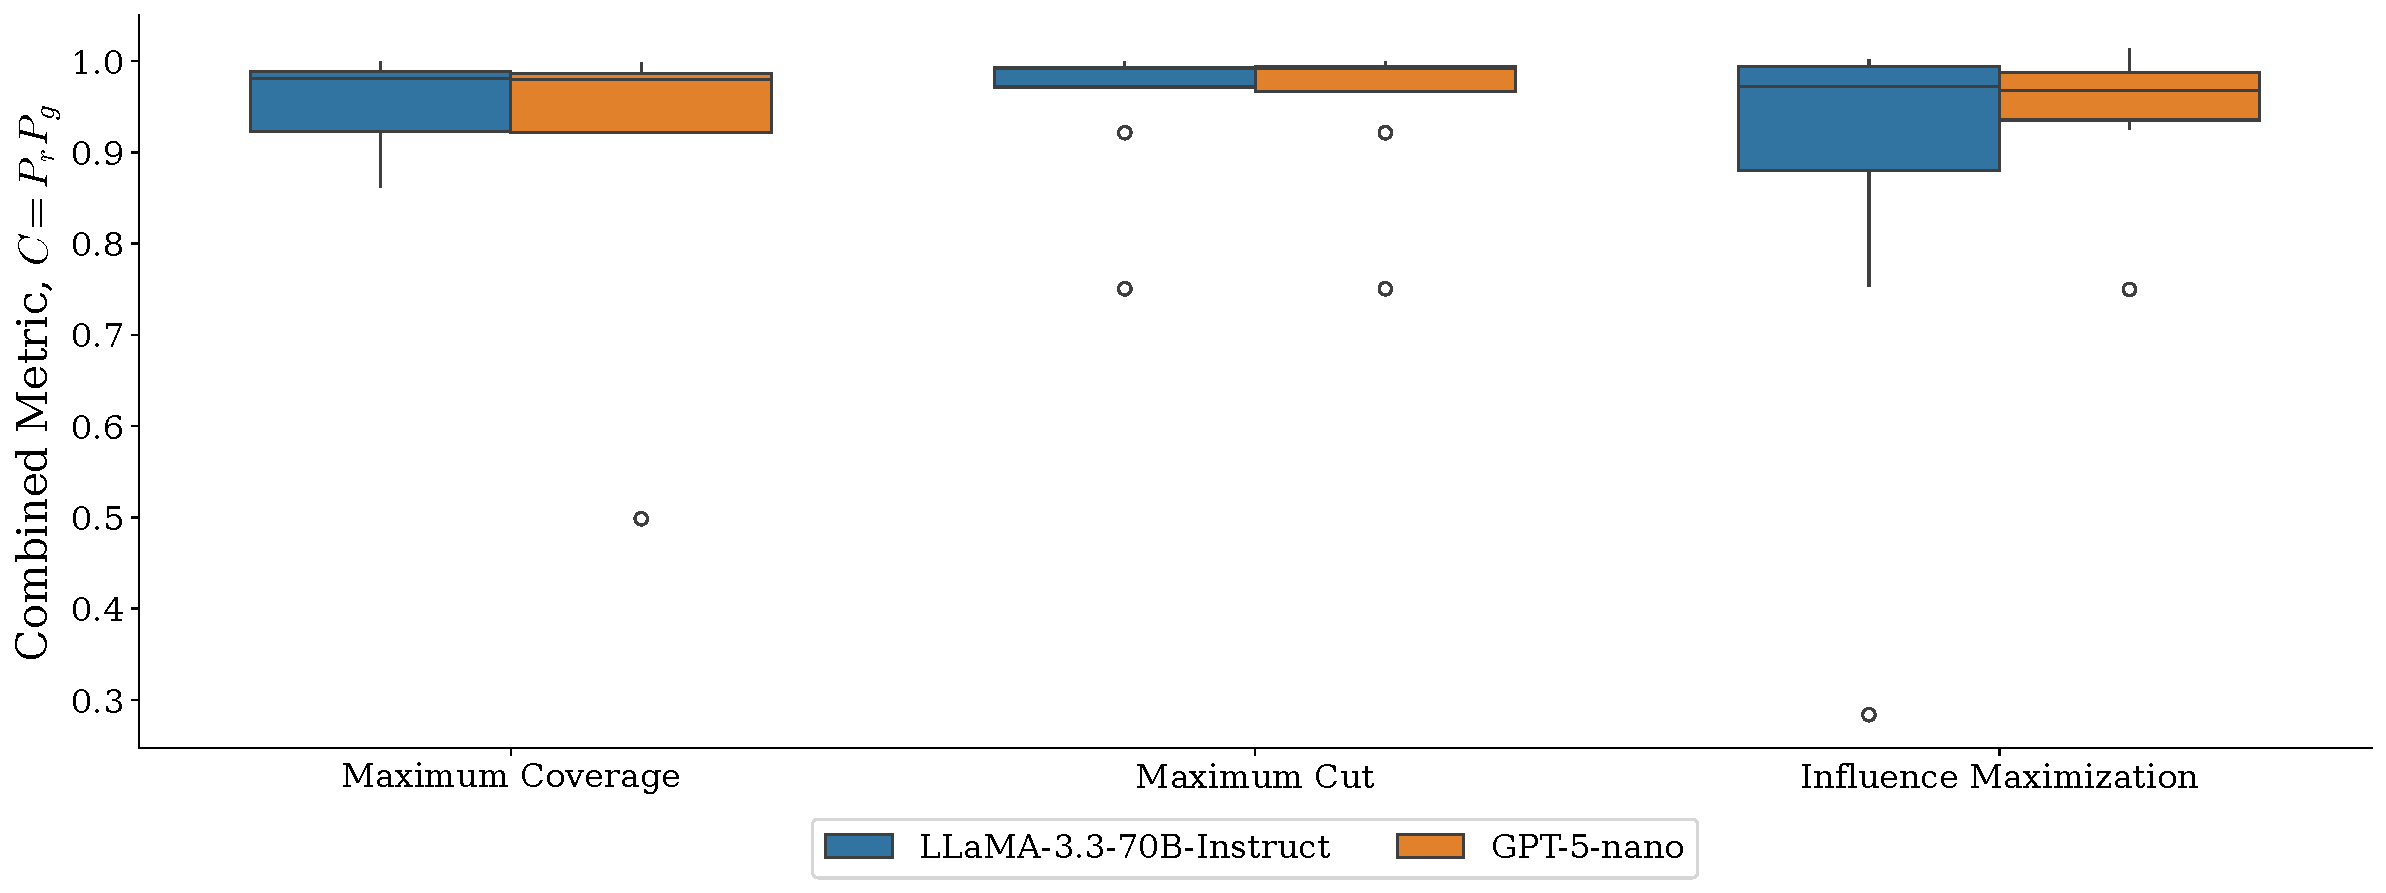
\includegraphics[width=\linewidth]{figures/models.pdf}
    \caption{Comparison of \llm using different LLMs. The plot shows the combined performance metric across all graph optimization tasks under constraints. Both GPT-5-nano and LLaMA-3.3-70B-Instruct yield similar performance, demonstrating that \llm is robust to the choice of the underlying LLM.}
    \label{fig:models}
\end{figure}